\documentclass[MS]{dukedissertation}

%%%%%%%%%%%%%%
% temp additions for notes
\usepackage{todonotes}
\usepackage[top=1.5cm, bottom=1.5cm, outer=5cm, inner=2cm, heightrounded, marginparwidth=3.5cm, marginparsep=1cm]{geometry}
%%%%%%%%%%%%%%



\usepackage{fontspec}
\defaultfontfeatures{Numbers=OldStyle}
\setmainfont{Minion Pro}


\usepackage{amsmath, amssymb, amsfonts, amsthm}
\usepackage{graphicx}
\usepackage{natbib}
\usepackage{color}
\usepackage{bm}
\usepackage{subfigure}
\usepackage{graphicx}
\usepackage{mathabx}
\usepackage{multirow}
\usepackage{setspace}
\usepackage{booktabs}
\usepackage{adjustbox}

\renewcommand{\bibname}{References}
\graphicspath{{./Pictures/}}

\author{Amogh Uday Karnik}
\title{Design and Usability Testing of  Mobile Phone-Based Patient Management System for Women in Rural Kenya}
\supervisor{Eric Green}
\department{Duke Global Health Institute}


\date{2014} % Year

% Copyright text.  If undefined, default is 'All rights reserved'
% (Example sets the text to a hyperlinked Creative Commons Licence)
\copyrighttext{ All rights reserved except the rights granted by the\\
   \href{http://creativecommons.org/licenses/by-nc/3.0/us/}
        {Creative Commons Attribution-Noncommercial Licence}
}

% Committee Members other than supervisor.  No more than five beyond the supervisor allowed.
\member{Nimmi Ramanujan}
\member{Lavanya Vasudevan}

\usepackage[xetex,bookmarks=true,colorlinks, linkcolor=black,urlcolor=black,citecolor=black, linktoc=section,]{hyperref}


\begin{document}

%-----------------------------------------------------------------------------%
%Title Page
%-----------------------------------------------------------------------------%
\maketitle

%-----------------------------------------------------------------------------%
%Abstract
%-----------------------------------------------------------------------------%
\abstract

\paragraph{Each year, more than 300,000 of women die from complications related to pregnancy, childbirth, or abortion. At least eighty percent of these deaths can be prevented by a set of proven interventions provided by a skilled practitioner, and two-thirds of all infant deaths can be prevented with antenatal care provided by a health professional during the first six weeks after delivery. However, delays in recognizing the need to seek care, delays in reaching health care facilities, and delays in receiving adequate care can all make delivery of the aforementioned interventions extremely challenging. Baby Monitor -  a novel, mobile-phone based screening system – hopes to help pregnant women and new mothers overcome these barriers to accessing care. In its current iteration, women listen to pre- and post-natal screening questions in their local language and respond by pressing keys on their mobile phones. The proposed research will focus on expanding the scope of this service by using the screening information to send patients health information, make referrals to local health facilities based on patient needs, and dispatch community health workers for targeted home visits. The development and testing of these features will ultimately lead to a system that helps address the delays in receiving effective in maternal and child health care and complements the existing health care system in Kenya.}} %Path to abstract.tex

%-----------------------------------------------------------------------------%
%Frontmatter: Table of Contents, List of Tables, List of Figures, List of Abbreviations
%-----------------------------------------------------------------------------%
\tableofcontents % Automatically generated
\listoftables	% If you have any tables, automatically generated
\listoffigures	% If you have any figures, automatically generated
%\abbreviations

% You can put here what you like, but here's an example
%Note the use of starred section commands here to produce proper division
%headers without bad '0.1' numbers or entries into the Table of Contents.
%Using the {\verb \begin{symbollist} } environment ensures that entries are
%properly spaced.

%\section*{Symbols}
%
%Put general notes about symbol usage in text here.  Notice this text is
%double-spaced, as required.
%
%\begin{symbollist}
%	\item[$\mathbb{X}$] A blackboard bold $X$.  Neat.
%	% Optional item argument makes the symbol/abbr
%	\item[$\mathcal{X}$] A caligraphic $X$.  Neat.
%	\item[$\mathfrak{X}$] A fraktur $X$.  Neat.
%	\item[$\mathbf{X}$] A boldface $X$.
%	\item[$\mathsf{X}$] A sans-serif $X$. Bad notation.
%	\item[$\mathrm{X}$] A roman $X$.
%\end{symbollist}
%
%\section*{Abbreviations}
%
%Long lines in the \texttt{symbollist} environment are single spaced, like in
%the other front matter tables.

\begin{symbollist}
	\item[CHV] Community health volunteer
	\item[CHEW] Community health extension worker
	\item[IVR] Interactive voice response
	\item[MAMA] Mobile Alliance for Maternal Action
	\item[mHealth] Mobile health
	\item[m-Pesa] Mobile money service utilized in Kenya
	\item[SMS] Short message service, used interchangeably with text messaging service
	\item[VoIP] Voice over Internet Protocol
\end{symbollist}
} % List of Abbreviations. Start file with '\abbreviations'

%-----------------------------------------------------------------------------%
% ACKNOWLEDGEMENTS -- included file should start with '\acknowledgements'
%-----------------------------------------------------------------------------%
%\include{{./Acknowledgements/acknowledgements}}

%=======================================%
% MAIN BODY OF PAPER
%=======================================%

%-----------------------------------------------------------------------------%
% Chapter 1: Overview
%-----------------------------------------------------------------------------%
%\chapter{Overview}

\paragraph{Each year, more than 300,000 of women die from complications related to pregnancy, childbirth, or abortion. According to the WHO, most maternal deaths occur between the third trimester and the first six weeks after delivery, with the most common causes being severe bleeding, hypertensive diseases, and infections \citep{WHO2012}. Moreover, the burden of maternal mortality is greatest among developing countries where most poor women deliver at home. In sub-Saharan Africa, one in every sixteen women will die of pregnancy-related causes - a lifetime risk higher than anywhere else in the world \citep{Ronsmans2006}.}

\paragraph{Most maternal deaths are avoidable. At least eighty percent of maternal deaths can be prevented by a set of proven interventions provided by a skilled practitioner, while two-thirds of all infant deaths can be prevented with antenatal care provided by a health professional during the first six weeks after delivery. However, delays in recognizing the need to seek care, delays in accessing  health care facilities, and delays in receiving adequate care can all make delivery of the aforementioned interventions extremely challenging \citep{Thaddeus1994}.}

\paragraph{These delays disproportionately affect women and families living in rural or remote regions. Community health workers or other health care professionals are few and far between in these areas, and complications that go unnoticed or are not treated early can prove to be deadly. The traditional solution to this challenge has been to increase the number of lay personnel, but there are many barriers to training and retaining human resources. A new automated screening and referral system called Baby Monitor is attempting to overcome this barrier by taking clinical screening directly to women using mobile phones. Women listen to screening questions in their local language and respond by pressing a key. Baby Monitor assesses responses and, when fully operational, will send information, make referrals, and dispatch community health workers.}

\paragraph{Over the past decade, mobile phones have had an incredible impact on low to middle income countries. Mobile phone technology has allowed millions of people to communicate to and from some of the most poor and remote areas of the world - especially in sub-Saharan Africa \citep{Adler2007}. In recent years, as mobile phone penetration has continued to increase, the use of mobile technologies for health monitoring and management has also become increasingly popular. Specifically, studies have shown that mobile applications may be the most promising way to improve disease prevention and management, especially in developing countries\citep{ColeLewis2010}.}

\paragraph{Text messaging, due to its availability, low cost, and instantaneous nature, has been by far the most popular intervention used in mobile health programs. Previous literature has focused on text message reminders and their utility for improving health seeking behaviors \citep{ColeLewis2010}, clinical attendance \citep{Guy2012},  adherence to antiretroviral regimens for patients with HIV \citep{Horvath2012}, and self- management of diabetes care\citep{Krishna2008}. Although data remains relatively scarce, meta-analyses on each of the previously described areas have shown that text messaging interventions can have a positive impact on health behaviors and outcomes.}

\paragraph{Mobile health initiatives have also focused on maternal and child health albeit in a limited context. Most of the current literature on mobile health for maternal and child health has focused on using mobile health interventions, such as text messaging, to educate intermediate health care providers. A 2012 systematic review of 34 different studies on mobile health interventions for maternal child health revealed that the majority of research initiatives have targeted community health workers, skilled birth attendants, and midwives \citep{Tamrat2012}. Other studies have explored how text messaging can be used to educate midwives, birth attendants, or community health workers in rural areas \citep{Woods2012}.}

\paragraph{The few initiatives that have focused on mothers as end-users, instead of health care providers, have also used text messaging as a means for education. The Mobile Alliance for Maternal Action (MAMA), a partnership between USAID and Johnson \& Johnson, has used text messages as the main tool to provide women with health information \citep{McCartney2012}. MAMA is a free text messaging service that provides educational information to women during pregnancy and one year post-delivery. This program has been implemented in several developing countries, including India, South Africa, and Bangladesh, and has been customized for each target region based on the known cultural norms and beliefs regarding pregnancy and child care \citep{McCartney2012}. These programs may also help improve the overall patient experience for pregnant women who have opted to receive prenatal care. Studies have shown that pregnant women who received biweekly text messages offering support during the time between prenatal care visits had higher satisfaction levels with their care than women who did not receive any messages in between visits \citep{Jareethum2008}.} 


\section{Fieldwork Site}
Eldoret, Kenya is very beautiful.

\section{Research Methods}
Methods were rigorous.}


%-----------------------------------------------------------------------------%
% Chapter 2: Manuscript'
%-----------------------------------------------------------------------------%
\chapter{Academic Manuscript}

\section{Abstract}
\textsc{Background:} Background was comprehensive.\\
\textsc{Objective:} Objective wasn clear. \\
\textsc{Methods:} Methods were complex.\\
\textsc{Results:} Results were promising. \\\
\textsc{Keywords:} maternal health, infant health, mHealth, patient referral, health informatics
\section{Introduction}
This section can include background information such as theories, prior work, and hypotheses. 
If this section is quite lengthy, use of subheadings are encouraged to break up the material logically. Subheadings should be consistent; therefore a subheading for the first part of the Methods section, for example, is also necessary (see below).

\section{Methods}

\paragraph{The development process for the patient management component of Baby Monitor was driven by the philosophy\todo{hmmm, philosophy sounds not scientific maybe philosopy and methods?} of human-centered design. Within this framework, a product is iteratively designed specifically with the end-users' \todo{add needs}behaviors and preferences in mind, so as to create a system that is easy to learn and intuitive to use \citep{Oviatt2006}. In this case, CHVs were identified as the primary end users for a potential patient management system given their critical roles within the Kenyan health system.}\todo{i'd make this last sentence a new paragraph and describe the kenyan system in a few sentences. alternatively, and maybe preferably, add this to the introduction. if you do the latter, this sentence will have context.}

\paragraph{The first phase of the design process sought to understand how people and information flow within the currently existing health infrastructure.\todo{could use a ``for instance'' here} This phase also aimed to identify areas of need or difficulty for CHVs and nurses in completing their jobs that could be addressed by a potential patient management system. The second phase of the design process was focused on development of a mobile phone-based system that would address the challenges and needs identified in phase one and improve communication between patients, CHVs, and nurses so as to improve overall health outcomes. The third and final phase of the process focused on the evaluation of the system by the stakeholders themselves through a mobile phone-based usability survey.}\todo{placeholder here for possible addition of use metrics}

\subsection{Setting}

\paragraph{The study was centered at Sinoko Dispensary, a rural Level 2 health facility in the Ndivisi Division of Bungoma East District in Western Province, Kenya\todo{i think we need to reference the new units that came out of the new constitution. provinces have been dissolved. counties are the new first level. we are in bungoma county. ndivisi is still the division.}. Located approximately 2km off of the nearest paved road, Sinoko Dispensary is one of only three public health facilities in the area \todo{define} equipped to handle deliveries. The two remaining facilities - Webuye District Hospital and Webuye Health Center - are located within the nearby town of Webuye, located at the southwestern border of the Division.}\todo{include distance}

\subsection{Recruitment}
\paragraph{For nurses and CHVs to participate in the study, they were required to be comfortable speaking in both English and Swahili and comfortable using a mobile phone to receive calls and text messages.}

\paragraph{At the time of recruitment, the staff at Sinoko included one clinical officer, who served as the head administrator, and four nurses.\todo{maybe a footnote to explain positions. not all nurses had same level.} 55 CHVs also reported to Sinoko at least once per month to provide information on the families living in their villages within the Sinoko catchment area.\todo{define and talk about community units as part of community strategy} Of these providers, three nurses and six CHVs, each representing a different village, were selected to participate based on the inclusion criteria and interest in the project. Upon selection, verbal and written informed consent was obtained from the nurses and CHVs prior to study participation.}

\subsection{Phase One - Relevance}\todo{i wonder if we should use the same HCD headings: hear, create, deliver...always good to anchor in terms of methodology}
\paragraph{In order to better understand the role of CHVs local to Sinoko, two focus group discussions were conducted at the clinic with the six CHVs selected to participate in the study. In the first discussion, the CHVs were asked to describe their daily workflow, discuss their experiences working with pregnant women and new mothers, and detail their administrative responsibilities. They were also asked to identify the most challenging aspects of their jobs as CHVs and to describe some of the local attitudes and perceptions related to pregnancy and maternal and child health. The second discussion was more focused on the concept of patient referral. Participants were asked to collectively describe their ideal system of communication between patients, CHVs, and nurses at the clinic. Audio from these discussions was recorded and analyzed for potential themes for design features for the patient management system. }

\paragraph{After the focus group discussion, field visits \todo{i think this needs to be more active to represent what you did. really shadowing, right?}were scheduled with two of the participating CHVs on separate dates. The purpose of these visits was to gain a better understanding of the CHVs daily responsibilities and to identify potential ways for the patient management system to fit into their existing workflow. Number of patients seen per day, amount of time spent with each patient, primary concern or chief complaint, and patient referral status (i.e. whether the patient was referred to Sinoko or scheduled for a follow-up home visit from the CHV) were documented for each patient visited over the course of the day.}

\paragraph{The final element of this design phase was a focus group discussion with the Sinoko clinic nurses selected to participate in the study. They were asked to describe their work responsibilities at the clinic, their experiences working with pregnant women and new mothers, and their interactions with the local CHVs. Like the CHVs, the nurses were also asked to  describe their ideal system of communication between patients, CHVs, and the clinic. This discussion was also recorded and analyzed to identify themes and design principles.}


\subsection{Phase Two - Development}\todo{if you introduce IVR at the end of the intro, then can assume reader remembers here. note that i am adding text directly to the document.}
\paragraph{With an understanding of user needs, behaviors, and preferences, we began the process of developing the referral component of Baby Monitor. The Baby Monitor service integrates several technologies: Verboice, a platform for designing and initiating automated phone calls over the internet; a Voice Over Internet Protocol (VoIP) provider in Kenya; a software framework called Asterisk used to connect Verboice to the VoIP provider; a telecommunications company in Kenya that delivers the automated call to the mobile handset of the end-user; a local SMS\todo{be sure to define earlier} gateway provider that sends text messages to end-users; and an analysis engine to process call data and trigger new calls from Verboice and send text messages from the SMS gateway provider. SOMETHING ABOUT INTEROPERABILITY.} 

\todo{i'd recommend mini-headings for each component}\paragraph{The system was designed in Verboice, an open source platform for creating projects that interact with end-users via voice and text, and R, an open source statistical computing environment. Verboice allows end-users to listen to audio messages in multiple languages, respond to questions with the phone keypad, and  record their own voice messages. Using the web-based Verboice platform, the research team built upon the existing Baby Monitor platform to create call flows designed for use by CHVs at Sinoko. Each call flow consisted of a series of instructions, questions, and prompts that require numeric input from the user's phone keypad, and was designed to address the design principles and themes identified for the patient management system during the first phase of the design process. For questions that required a 'yes' or 'no' answer, users were asked to press '1' or '3' on their keypads. For other questions, users were also asked to enter numerical data through their keypads. No data or answers to questions were stored locally on their phones; all responses to all questions were saved to the research team's Verboice database.} 

\paragraph{The research team also created a set of text messages specific to the roles and responsibilities of the CHVs in order to supplement the interactive voice response system. These messages were designed to use information provided by the CHVs in previous calls with the system to help them complete their daily responsibilities. Additionally, the research team adapted a set of text messages from the Mobile Alliance for Maternal Action (MAMA) designed for pregnant women and new mothers. Both sets of text messages were automated through an R script written for the larger Baby Monitor project, which also automated calls to the CHVs through Verboice.}

\paragraph{In order to test these call flows and automated text messages, the research team conducted a mock testing session with the CHV focus group. Index cards with text were used to represent each audio or text message, and volunteers were selected to read the messages aloud to the group. This was done in order to confirm the content and logical flow of the messages and questions, and to gain feedback on the strengths and weaknesses of the system. Based on feedback from this focus group session, the research team finalized the content and flow of each message in the call flow within the web-based Verboice platform. A woman native to Ndivisi and familiar with the local dialects was recruited to assist in translation of all messages and recording of the audio messages in English and Swahili. Recording was completed at A STUDIO IN A NEARBY TOWN.}


\subsection{Phase Three - Evaluation}
\paragraph{The three nurses previously selected to participate in the study and the full sample of 55 CHVs were chosen to pilot the patient management system with patients within the Sinoko catchment area. The primary outcomes for this evaluation phase were frequency of use of the system and user-determined\todo{replace with self-reported} usability rating. Data regarding the use of the patient management system was collected over the course of six months, after which usability testing was initiated. A modified version of the Health IT Usability Evaluation Scale \citep{Yen2010} was administered to all CHVs through a Verboice call flow (SEE FIGURE INSERT FIGURE REFERENCE, OR TABLE). Participants were called through Verboice via an automated R script and listened to a series of statements regarding the quality of work life, perceived usefulness, and perceived ease of use of the system. Using their numeric keypads, they were asked to press '1' to agree with the statement and '3' to disagree. They were subsequently asked to whether they agreed or disagreed 'a lot' or 'a little'. This modified Likert scale allowed for a quantification of the system's overall usability and identification of weaknesses in the current system design.\todo{since we could have asked them to use the keys 1-4, design was not a limitation. ease of understaning and administration was the reason.}}



\section{Results}
\paragraph{Throughout the relevance and development phases\todo{consider changing phase labels as noted in methods section}, the CHVs and nurses emphasized three key priorities for the design of a potential patient management system: communication from the CHV to the clinic, communication between the clinic and the CHV, and reminders for CHVs to help them keep up with their myriad of responsibilities on a day to day basis.}\todo{With changes to structure of the section, this opening sentence needs to be revised.} 


\subsection{Hear Phase}

\subsubsection{Reporting Home Visits}
\paragraph{CHVs described conducting home visits with patients as their major responsibility. They made rounds in their village at least one day per week, depending on their own work schedules. Number of households visited varied per week, but participants in the focus group collectively concluded that it took approximately 5-6 months to complete rounds at every household in their village before beginning again. Every two weeks, CHVs were required to visit the health facility to submit reports detailing a number of demographics - including number of pregnant women, number of infants under six months of age, number of children under age five, number of births, and number of women provided with family planning information and materials. These reports are then compiled for each month by the CHEWs\todo{i think this is the first this appears. introduce earlier, but even then, i suggest replacing acronym with the word supervisor.}. Members of the focus group were unable to describe what type of analysis or evaluation took place after submission of their reports, and some questioned whether any oversight of the reported data took place.\todo{modify this description by deleting the part after the comma} Table~\ref{tab:chvreport2013} shows selected indicators collected by CHVs in the study catchment area during the first six months of 2013. }

\paragraph{During field visits \todo{consider a different name of activity as mentioned earlier}with the research team, the CHVs described the reporting process as difficult and somewhat disjointed. Both CHVs observed took minimal notes when making home visits, instead opting to complete their log sheets at the end of the day\todo{do we know why?}. During the field visit days, the CHVs and research team met with four and five households respectively. Time spent at each household varied based on the family's concerns and size of the family, but lasted anywhere from fifteen minutes to one hour. Both CHVs carried 'referral books', which contained a series of carbon-copied sheets with spaces for the date, patient name, and chief complaint to be completed by the CHV. Each sheet had three copies: one for the CHV, one for the patient, and one to be kept at the clinic. However, both CHVs indicated that they rarely kept their copy of the referral sheets\todo{any insight into why...e.g., no way to keep records?} and were unable to show the research team any sheets from previous referrals.}

\paragraph{Discussion with the clinic nurses offered additional insight into the nature of CHV home visits. They noted that the CHVs submitted reports that were compiled monthly by the CHEWs. However, the nurses indicated that they rarely looked at the monthly CHV log books to track patient visits. Instead, the main indication of CHVs conducting home visits was the presence of patients with referral slips from their CHVs. The nurses reported that they received approximately 50 CHV referrals per week\todo{meaning slips? seems high for actual slips. if correct, let's put in terms of weekly patient volume}, with an estimated 15 being related to antenatal care visits. They also indicated that patients rarely came in with both copies of the CHV referral sheets, making it difficult to completely track the flow of referrals from CHV to clinic accurately.}

\paragraph{Based on these findings, the research team designed a fast and simple method of reporting home visits to pregnant women and new mothers within a Verboice call flow. After completing a visit, the CHV flashes\todo{have you described this? include in the methods section} the Baby Monitor number and receives a free incoming call from the system. After indicating that they are a CHV and identifying themselves with their unique ID number, they are asked to \todo{to select from a menu of options that includes reporting a home visit}confirm that they would like to report a home visit. They are subsequently asked to identify the household they have visited by \todo{entering the phone number the woman provided at enrollment...we also need to describe somewhere how the CHV gets the woman's number.} their phone number. After confirming the phone number, they are asked to indicate the date of the visit by pressing '1' for the current day, '2' for the previous day, and '3' for another date\todo{before yesterday}. If they select another date, they are asked to input the month and date (following separate prompts) using their keypads. This information is saved in the Baby Monitor database, and the call is completed.}


\subsubsection{Referral Notifications}
\paragraph{The CHV focus group agreed that the majority of their home visits concluded with a patient referral to the clinic. However, they also indicated that they had no way of knowing whether a patient followed up on that referral until their next visit to the household weeks or even months later. Most of these referrals were for routine prenatal visits for pregnant women. The CHVs indicated that most women did not follow up on routine prenatal care referrals due to the costs of the care and travel to the clinic. However, on June 1, 2013, President Uhuru Kenyatta declared that all public health facilities would provide free care to all pregnant women. While uncertain about its implementation, the CHVs were hopeful that this policy would drive more women to follow up on their referrals. }

\paragraph{During the CHV shadow days, two women were identified as having missed a previous referral for prenatal care. The first woman had been referred three months before, but had since delivered a healthy baby at home without receiving any prenatal care. The second woman had been referred over six months before, and now had a healthy four month-old child. However, she hadn’t had a regular menstrual cycle in two months and the CHV suspected that she may be pregnant again. After visiting with this woman and making a referral to the clinic, the CHV expressed regret at not visiting this woman sooner. }

\paragraph{Based on these results, the research team designed a text-message based system to provide CHVs with notifications when pregnant women in their villages visited the clinic.  As part of the larger Baby Monitor project, pregnant women who visited the clinic were asked to enroll in the Baby Monitor system. Any visit from an enrolled woman was logged by the clinic nurses. At the end of each day, this data was entered via FormHub, a mobile phone based data entry tool, into a secure server accessible only to the research team. An R script was written to use this data to match each woman who visited the clinic that day to the CHV assigned to their village. The script was automated to send text messages every morning to the corresponding CHVs, informing them that women from their village had visited the clinic the previous day.}

\subsubsection{Reporting Home Deliveries}
\paragraph{Both the CHV and nurse focus groups indicated that most pregnant women in this region delivered at home. Some of these women opt to deliver with their CHVs present, but many also use the services of birth attendants who assist in the delivery process in the woman's home. CHVs indicated little trouble in identifying home deliveries for reporting, as word of a new birth usually spread through the village quickly. The CHVs emphasized that word of mouth and speaking with community members was an especially important way for them to identify individuals who may require care. On the first field visit day with the research team, the CHV visited two new mothers after hearing from another community member that they had given birth within the past two months. Although the CHVs acknowledged a potential time delay in identifying deliveries by word of mouth, they collectively agreed that most deliveries were reported relatively soon after taking place.}\todo{within the first day? need to be more specific here. cases observed are very late. even best case scenario might be outside of window when most maternal and neonatal deaths occur.} 

\paragraph{The clinic nurses indicated that the only report of home deliveries they receive are on the CHV monthly reports, which they previously acknowledged to using very rarely. They attributed the preference to deliver at home to cost of travel to Sinoko, and also indicated that not regularly checking for the number of recent deliveries presents challenges for providing postnatal care to women and children who may need it at the clinic.}

\paragraph{To address these findings, the research team designed a call flow similar to that of reporting CHV home visits for reporting deliveries. After flashing the Baby Monitor system and identifying themselves as CHVs, the CHV is asked to identify the woman who has delivered by her phone number. Date of delivery is indicated by pressing '1' for the current day, '2' for the previous day, and '3' for another date, which is input directly using their keypads. This delivery information is saved into the Baby Monitor database, and the call is completed.}



\subsubsection{Delivery Notifications}
\todo{How do we notify CHVs of deliveries that they may not be aware of? This section still to be determined.}%%%%%%%%%%% EDIT %%%%%%%%%%%

\paragraph{For home deliveries, the research team created an identical delivery reporting call flow to be used by the new mothers or their family members. After flashing the Baby Monitor system and opting to report a delivery as, the user is asked to identify the new mother by her phone number. Date of delivery is indicated by pressing '1' for the current day, '2' for the previous day, and '3' for another date, which is input directly using their keypads. This  information is saved into the Baby Monitor database, and the call is completed. For deliveries at the clinic, all successful deliveries by enrolled women were logged by the clinic nurses. This logged data was entered via FormHub and stored in the Baby Monitor database. Using both sources of information, the clinic visit notification system was adapted to instead provide delivery notifications. In a similar manner, text messages were sent to CHVs every morning, informing them of deliveries that took place on the previous day.} 


\subsubsection{Reporting Emergencies}
\paragraph{The CHV focus group identified emergency reporting as a major area of concern in their existing workflow. CHVs reported that they were usually called by a family member during a health-related or pregnancy-related emergency. In most cases, they recommended that the patient travel to Sinoko\todo{i'd refrain from using the clinic name throughout this document, even in the setup section} to receive care at the clinic. However, they noted numerous occasions in which the patient arrived at Sinoko, only to find the clinic understaffed at that time of day or unprepared to handle certain emergency procedures due to limited medical supplies. The group attributed this to a lack of direct communication between the CHVs and the clinic, indicating if they knew that the clinic was not prepared for an incoming patient, they could refer and accompany the patient to another clinic or Webuye District Hospial\todo{same here. refer to closest level 3 facility}. They also indicated that news of these missed emergencies contributed to an unwillingness to visit Sinoko among community members. This perception was reflected during both field visit dates, as three separate pregnant women expressed some concern about delivering at Sinoko due to a combination of cost and prior missed emergencies.}

\paragraph{Discussion with the clinic nurses also reflected concerns about emergency reporting and referral to the clinic. The nurses acknowledged that there was little to no direct communication between CHVs and the clinic staff about incoming emergencies. Pregnant women often came to deliver with little prior notice at any time of the day, making it difficult for the nurses to prepare for their care. The nurses indicated that only one nurse is typically on call overnight, and at least two nurses are needed to complete a safe delivery procedure. Moreover, the nurses indicated that the clinic has capacity for only three deliveries per week due to limited supplies. If more than three women came into the clinic for a delivery, they would have to wait for an ambulance to arrive from Webuye to take them to the District Hospital in town.}

\paragraph{Based on these results, the research team designed a simple call flow to be used by patients, family members of patients, and CHVs to report an emergency to a nurse on staff at Sinoko clinic. The user flashes the Baby Monitor system, and indicates that they would like to report an emergency. After confirming that the user would like to speak directly to a clinic nurse, the system forwards the call to the clinic phone, free of charge to the user. The user can then describe the emergency to the nurse at the clinic, and the nurse can advise the patient, family member, or CHV on how to proceed. This allows the nurse to prepare for the arrival of the patient and call the other nurses to the clinic if necessary.}

\subsection{Create Phase}
\paragraph{Mock testing of the above features was focused on identifying key strengths and areas for improvement for the system. Participants of the focus group indicated that the system was straightforward and simple, and was designed to provide useful information for their daily responsibilities. Participants also noted that the text message notifications regarding completed referrals and deliveries at the clinic would be helpful in terms of data collection for their biweekly reports. In all, the CHVs agreed that the major design features of the system addressed their major areas of concern in regards to communication between CHVs, the clinic, and their patients.}

\paragraph{While the participants were optimistic about the potential of the prototypes demonstrated at the mock testing session, they also voiced concern about accessing the system via mobile phone. Participants indicated that a lack of credit on CHV phones would affect use of the system, as a minimal amount of credit is required for a user to flash a number. According to the group, most CHVs carried very little credit on their phones on a day-to-day basis, adding money only when necessary due to cost. Group participants suggested that use of the system would vary greatly, since some CHVs were better at maintaining credit and using their phones regularly than others. To address these findings, the research team opted to provide a 50 Ksh incentive for each home visit and delivery reported by participating CHVs, thus encouraging CHVs to maintain a minimal amount of credit in order to engage with the system.}


\subsection{Deliver Phase}
\subsubsection{Usability Testing Results}
\paragraph{Results of the usability testing survey were generally positive. Response rate was very high among participating CHVs; 53 out of 55 (96\%) of users responded to the survey. Results corresponding to each item of the usability evaluation scale can be found in Fig ~\ref{fig:barchart}. Perceived ease of use of the system was relatively high. 70\% of respondents strongly agreed that the overall system was easy to use, while 28\% moderately agreed and 2\%  moderately disagreed. }

\paragraph{Perceived usefulness of the system was very high. 100\% of respondents agreed that they liked receiving messages from the system. 100\% of respondents also agreed that the messages help them keep track of their clients, with 81.6\% strongly agreeing with this notion. 98\% of respondents agreed that the system saved them time, 81.6\% of which strongly agreed.}

\paragraph{Respondents indicated that interacting with the system was relatively simple.  Approximately 96\% of respondents agreed that it was easy to report a home visit, while 2\% moderately disagreed and 2\% strongly disagreed. Similar trends emerged for respondents' evaluation of the delivery reporting system. 96\% of respondents  agreed that delivery reporting was easy, while 2.0\% moderately disagreed and strongly disagreed. Ease of use for emergency reporting was slightly lower. 94\% of respondents agreed that emergency reporting was easy, while 6\% disagreed. The text messaging elements of user interaction were rated very highly among respondents. 100\% of respondents agreed that the messages were easy to understand, and 100\% also agreed that the messages were usually accurate.}

\paragraph{Finally, quality of work life with the system was rated to be relatively high. 94\% of all respondents (76\% strongly agreeing and 18\% moderately agreeing) believed that the system helped them do their jobs as CHVs better than before.}


\begin{figure}[h]
	\begin{center}
	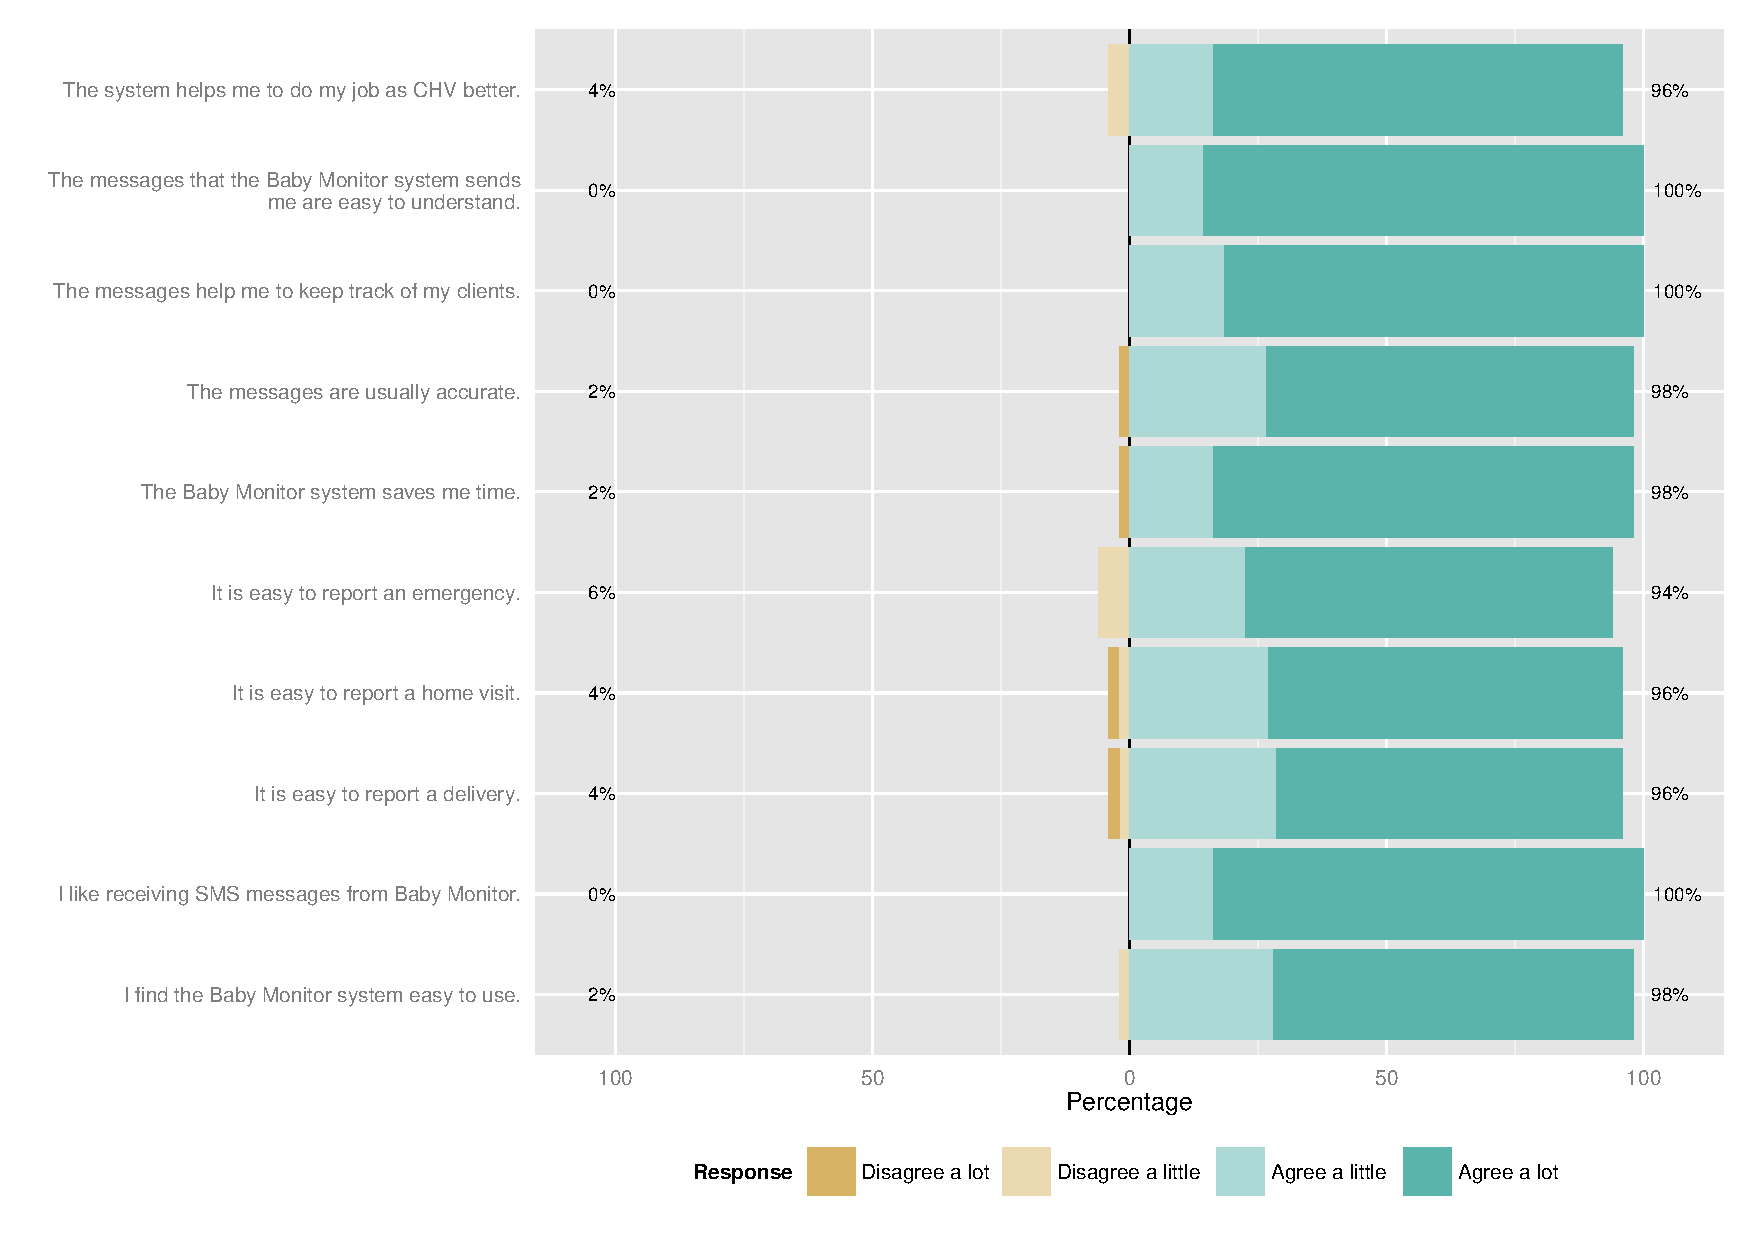
\includegraphics[height=4.5in]{usability-bar-316}
	\end{center}
	\caption[Usability survey results]{CHVs generally found the service to be usable. The SMS messages sent by the system were among the highest rated features of the system. Overall, 94\% of respondents believed that the system helped them do their jobs as CHVs better than before.}
	\label{fig:barchart}
\end{figure}


\section{Discussion}

\subsection{Principal Results}
\paragraph{The Hear phase revealed three general areas in which the CHVs were involved in maternal and child health care: home visits with pregnant women and new mothers, monitoring new deliveries in the community, and emergency care. Within each of these areas, three key themes emerged as priorities for the CHVs in designing a new patient management system: the need for fast, easy, data reporting methods, improved communication between CHVs and the clinic regarding referrals, and the need for an effective, reliable way to report and respond to obstetric emergencies. These themes led to the inclusion of five key design features that complemented the daily tasks of CHVs in the study catchment area, which are outlined as follows:}
\begin{enumerate}
	\item Reporting of home visits through IVR
	\item Notification of referred patients visiting the clinic through text message
	\item Reporting of deliveries through IVR
	\item Notification of patients delivering at the clinic through text message
	\item Reporting of emergencies directly to the clinic through IVR
\end{enumerate}

\paragraph{Mock testing of these features during the Create phase revealed enthusiasm and satisfaction with the service, but concerns were raised regarding the ability for CHVs to flash the Baby Monitor phone number should they run out of phone credit. This issue was addressed by including m-Pesa payments, which can be transferred directly into phone credit, for CHVs participating in the study.}

\paragraph{CHVs generally found the system to be usable. The text messages notifying CHVs of patient visits and deliveries were among the highest rated features of the system. }\todo{This section to be updated once results are complete. - A}

\subsection{Limitations}
This study piloted an intervention that was previously untested in this target population. Thus, the scope of the study was limited to a single clinic and a small, convenience sample of CHVs working in the clinic's catchment area. Participants for focus groups were selected based on English comprehension and demonstrated interest in the study, and thus may not generally represent the perspectives or viewpoints of all other CHVs within the health system. Due to time contraints, only one cycle of the Hear and Create phases were completed; in future iterations, additional cycles of prototyping and mock testing would have been conducted in order to refine and create additional features for the system.  

\subsection{Comparison with Prior Work}

- MoTECH program: IVR/texts in Ghana for midwives
- Believe that this has potential to improve community-based maternal and child health care

\subsection{Conclusions}}

%-----------------------------------------------------------------------------%
% Chapter 3: Reflection
%-----------------------------------------------------------------------------%
%\chapter{Reflection	}

This chapter will  summarize the overall project, with a focus on lessons learned, implications for future research and intervention, and limitations. It can, but does not have to, include a more personal reflection on the research process. 


}


%-----------------------------------------------------------------------------%
% Appendices
%-----------------------------------------------------------------------------%
\appendix
\chapter{Usability Survey }


\begin{table}[htp]
  \centering
  \caption{Modified version of the Health IT Usability Evaluation Scale developed by \cite{Yen2010}.}
    \begin{tabular}{ll}
    \toprule
    \textbf{Concept} & \textbf{Item} \\
    \midrule
    \textit{Perceived Ease of Use} &  \\
    \textit{} & 1. I find the Baby Monitor system easy to use.  \\
    \textit{} & 2. It is easy to report a home visit. \\
    \textit{} & 3. It is easy to report a delivery.  \\
    \textit{} & 4. It is easy to report an emergency.  \\
    \textit{Perceived Usefulness} &  \\
    \textit{} & 5. I like receiving SMS messages from Baby Monitor.  \\
    \textit{} & 8. The messages help me keep track of my clients.  \\
    \textit{} & 9. The Baby Monitor system saves me time.  \\
    \textit{User Control} &  \\
    \textit{} & 6. The messages that the Baby Monitor sends me are easy to understand.  \\
    \textit{} & 7. The messages are usually accurate.  \\
    \textit{Quality of Work Life} & \textbf{} \\
          & 10. The system helps me to do my job as a CHV better.  \\
    \bottomrule
    \end{tabular}%
  \label{tab:usabilitysurvey}%
\end{table}%


}

%-----------------------------------------------------------------------------%
% References
%-----------------------------------------------------------------------------%
\bibliographystyle{./Bibliography/apalike} %Formats bibliography
\cleardoublepage
\normalbaselines %Fixes spacing of bibliography
\addcontentsline{toc}{chapter}{References} %adds References to your table of contents
\bibliography{./Bibliography/BabyMonitor} %your references file - change the path if needed



% temp
\listoftodos
































\end{document}
